\documentclass[language=en,11pt]{aghdpl}


\author{Aleksander Nagaj}
\shortauthor{A. Nagaj}

%\titlePL{Przygotowanie pracy dyplomowej w~systemie~\LaTeX}
\titleEN{Vision system for controlling the route of an autonomous boat using machine learning methods.}


%\shorttitlePL{Przygotowanie pracy dyplomowej w~systemie \LaTeX} % skrócona wersja tytułu jeśli jest bardzo długi
%\shorttitleEN{Preparation of a long and fascinating thesis in \LaTeX}


% Dopuszczalne wartości[1,2]:
% * "Projekt dyplomowy" - na koniec studiów I stopnia
% * "Praca dyplomowa" - na koniec studiów II stopnia
% [1] Zasady dyplomowania w roku akademickim 2020/2021 (Decyzja Dziekana WEAIiIB nr 16/2020 z dnia 9 grudnia 2020 roku)
% [2] Załącznik nr 1a) do Decyzji nr 16/2020 Dziekana Wydziału EAIiIB z dnia 09 grudnia 2020 r.
%\thesistype{Praca dyplomowa}
\thesistype{Bachelor of Science Thesis}

\supervisor{Maciej Rosół, PhD}

\degreeprogramme{Automatics and Robotics}

\date{2021}

\renewcommand{\contentsname}{Table of Contents}

\department{Department of Applied Computer Science}

\faculty{Faculty of Electrical Engineering, Automatics, Computer Science and Biomedical Engineering}

\acknowledgements{For Em}


\begin{document}
    % \setcounter{page}{1}

	\titlepages
	\RedefinePlainStyle
	
    \begin{abstract}
\setcounter{page}{3}
    Reinforcement learning methods are commonly used in various areas such as: self-driving cars, trading and finance, NLP\footnote{Natural Language Processing} and many more. Q-learning is an off-policy, model-free algorithm that found numerous applications in a training of autonomous agents. With a support of Deep Neural Network to evaluate and improve action policy, Deep Q-Learning became a powerful enough tool to teach an autonomous boat how to find a route using its vision system in an environment when it was trained. This paper gives a detailed information of how it was achieved and compares different architectures of DQN applied to solve the task given in the Thesis.
\end{abstract}


	
	\setcounter{tocdepth}{2}
	\tableofcontents
	\clearpage
	
	\chapter{Introduction}
\label{cha:introduction}

The recent development in the deep learning area has resulted in a significant increase in usage of artificial intelligence
solutions. Recommendation algorithms, voice or face recognition, type hinting - these are only examples of technologies which are
used on a everyday basis by millions. Deep Artificial Neural Networks are by far the most robust of all machine learning
algorithms capable of handling various tasks in an unprecedented manner. Thus the choice of getting hands on designing and
implementing vision system for an autonomous boat which uses their full potential.

\section{Purpose}
\label{sec:purpose}

The goal was to create a \textbf{vision system} for an autonomous agent which would be responsible for its autonomous control on a given
track limited by buoys. The system uses images retrieved from a pair of front cameras to train a \textbf{Deep Reinforcement Network}
responsible for track analysis and boat control. The entire project is held in a simulation environment where a designed algorithm is
trained on a boat model which resembles a real life counterpart. 

The expected result was a well-designed and trained Deep Reinforcement Network capable of controlling the boat within defined constraints.
Ideally the network should be tested in a real environment, however due to limited resources and time the overall performance was measured
entirely in the simulation.

\section{Real-life applications of Reinforcement Learning}
\label{sec:real-life-applications-of-deep-learning}

\subsection{Games}
\label{sub:intro-games}
RN nowadays is well-known due to algorithm which used to play different games and managed to achieve a super-human performance in some.
The DQN agent designed by \emph{Google Deep Mind} was able to play 49 different Atari 2600 games (\ref{fig:Atari2600}). However, the most
famous one is probably the \emph{AlphaGo} \cite{AlphaGO}  and \emph{AlphaGo Zero}. AlphaGo was trained on countless human games achieving
robust performance, but it was not sufficient for the researchers. They let their new agent trained from scratch - AlphaGo Zero to play with
itself and eventually beat AlphaGo 100-0. 

\begin{figure}[h]
    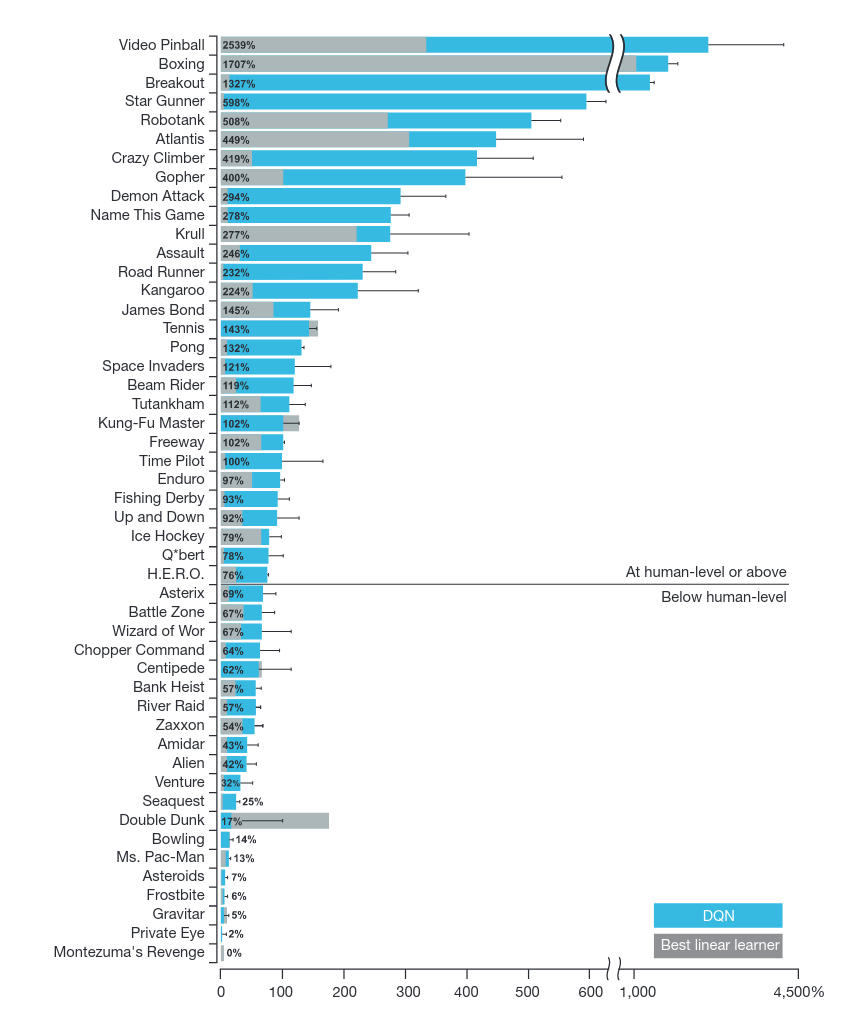
\includegraphics[width=10cm]{img/Atari2600.png}
    \centering
    \caption{Reinforcement Learning model vs human-level performance in the Atari 2600 environment \cite{DQNAtari}}
    \label{fig:Atari2600}
\end{figure}

\subsection{Robotics}
\label{sub:intro-robotics}
As stated in survey conducted by \emph{Jens Kober}, \emph{J.Andrew Bagnell}, and \emph{Jan Peters} \cite{RNSurvey}, ``\emph{Reinforcement
learning offers to a robotics a framework and set of tools for the design of sophisticated and hard-to-engineer behaviors}''. In fact, these
are most of existing ones in a real world. Instead of engineering a set of deterministic movements of a robot in a controlled environment,
identical or improved result can be achieved through training in a well-defined task which provides feedback measuring robot's performance.
Such approach enables to train robots for performing tasks in more real world environments which are not usually fully controllable.

\subsection{Personalized Recommendations}
\label{sub:intro-personalized-reccomendations}
News recommendations tends to be challenging due to the fact that most of the users easily get bored. Even if one clicks at the article,
there is a low likelihood that it will be read to the end. Therefore Click Through Rate standalone, which is used by many algorithms, is an
ineffective indicator. In order to improve the quality of recommendations and address this issue, the DQN was designed and described in
\emph{DRN: A Deep Reinforcement Learning Framework for News Recommendation} \cite{DRNNewsRecommendaiton}. This method uses multiple features
to determine what will be displayed to the user.

	\chapter{Deep Learning}
\label{cha:dl}

Machine learning methods are used widely for regression and classification problems. Contemporary companies in order to keep up with the pace of customers expectations rely heavily on such algorithms. They require human intervention to learn. Which is possible for relatively small data sets, but gets extremely complicated or even impossible for larger ones. \textbf{Deep learning (DL)}, however, solves that issue by eliminating the need of human supervision by automating feature extraction. These algorithms can leverage from labeled data sets but do not require them to function. Together with the scalability, DL methods are by far superior to any other Artificial Inteligence solutions. This sections gives an insight of how \textbf{Deep Neural Networks (DNN)}, which are the core of DL, are created.


\section{Neuron}
\label{sec:neuron}

Neuron is the most elementary part of the \textbf{Artificial Neural Network (ANN)}. The idea behind it was to emulate the behaviour of its biological counterpart. It consists of set of inputs $x_1, x_2, ..., x_n$ connected with digital synapses. Each of this connections is given a weight $w_1, w_2, ..., w_n$ representing an importance of the receptive inputs to the output. The output of neuron is determined by the \textbf{activation function} $\phi(x)$, which is described in more detail in the next section (\ref{sec:activation-function}). Where $x$ is the weighted sum of $\sum_j {x_j}{w_j}$ offset by bias $b$. To simplify, the weighted sum can be expressed as a dot product $x \cdot w$.

\begin{figure}[h]
    \centering
    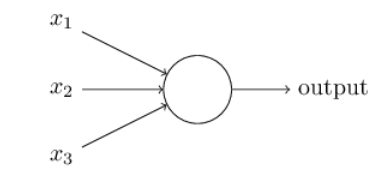
\includegraphics[width=8cm]{img/Perceptron.png}
    \caption{A neuron. Source \cite{NNandDL}}
    \label{fig:neuron}
\end{figure}

\section{Activation Function}
\label{sec:activation-function}

Every neuron in network, except inputs, consists of an activation function. In simple terms, it takes sum of weighted inputs and returns a value which tells how strong the neuron fires. In other words, the higher the activation function return, the stronger influence it has on the next layer. The return is usually within the range $[0, 1]$. Examples of activation functions are: 
\begin{itemize}
    \item Threshold \hspace{5pt}
        $\phi(x) = 
        \begin{cases}
            1 & x \ge 0 \\
            0 & x<0
        \end{cases}$
    \item Sigmoid \hspace{5pt}
        $\phi(x) = \frac{1}{1+e^{-x}}$
    \item Hyperbolic Tangent (tanh) \hspace{5pt}
        $\phi(x) = \frac{1-e^{-2x}}{1+e^{-2x}}$
    \item Rectifier Linear Unit (ReLU) \hspace{5pt}
        $\phi(x) = max(0, x)$
\end{itemize}

The most commonly used is undoubtedly the \textbf{ReLU}, which was proposed and researched by \emph{Xavier Glorot et al.} \cite{DeepSparseReNN}. It allows a network to easily obtain a sparse representation, which has numerous advantages and also mostly resembles neurobiological structures. Human brain is hypothesized to have 95\% to 99\% sparsity.

\section{General architecture of artificial neural network}
\label{sec:general-architecture-ann}

The leftmost layer of the network is called input layer and so are called the neurons that it consist of - \textbf{input neurons}. The rightmost output layer consists of, no surprise, \textbf{output neurons}. All the in-between layers are called \textbf{hidden}. At first glance, the term ``hidden'' may perhaps sound mysterious. However, there is not special meaning behind it. It could be as well called ``not an input or an output'' and be self-explanatory of what it actually is. A deep network is always made of an input, output and one or more deep layers.

\begin{figure}[h]
    \centering
    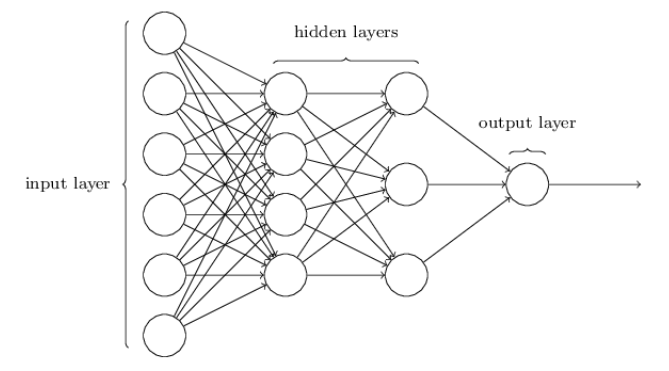
\includegraphics[width=12cm]{img/ANN-diagram.png}
    \caption{An artificial neural network. Source \cite{NNandDL}}
    \label{fig:ann}
\end{figure}

\section{Cost Function}
\label{sec:cost-function}

\subsubsection*{Notation}
\label{sub2:notation}

Before jumping straight into mathematical details, there should be a notation explained so it would not confuse anyone. The one was originally proposed by Michael Nielsen in ``\emph{Neural networks and deep learning}'' \cite{NNandDL}.

The \textbf{activation} (output) of the $j^{th}$ neuron in the $l^{th}$ layer is called $a^l_j$. Subsequently, the $j^{th}$ element of the input vector would be $a^1_j$. Now the relation between consequent layers outputs can be written down:

\begin{equation}
\label{eq:2.1}
a^i_j = \phi\left(\sum_k (w^l_{jk} \cdot a^{l-1}_k) + b^l_j\right)
\end{equation}

where $\phi$ is the activation function,

$w^l_{jk}$ is the weight from the $k^{th}$ neuron in the $(l-1)^{th}$ layer to the $j^{th}$ neuron in the $l^{th}$ layer,

$b^l_j$ is the bias of the $j^{th}$ neuron in the $l^{th}$ layer,

$z^l_j = \sum_k (w^l_{jk} \cdot a^{l-1}_k) + b^l_j$ is the activation value of the neuron before the application of activation function.

\vspace{.5cm}

For more concise notation let us write $a^l = \phi(w^l a^{l-1} + b^l)$, taking advantage of matrix and vector operations.

Having explained a notation, we can discuss what the cost function actually is. Briefly, it is a method of measuring of how good the neural network performed regarding given training sample and the expected output. The return of cost function is always a scalar value, since it indicates overall network performance. It can be written in a form of a following tuple

\begin{equation}
    C(W, B, S^r, E^r)
\end{equation}

where $W$ are network's weights, $B$ biases, $S^r$ is the input of a single training sample and $E^r$ is the desired output of a single training sample.

\subsubsection*{Requirements}
\label{sub2:cost-requirements}

In order to compute gradient, which is a key part of a DNN learning process, the cost function must satisfy following constraints:

\begin{enumerate}
    \item The cost function $C$ must be able to be written as an average
    
        \[C = \frac{1}{n} \sum_x C_x\]
        
        over cost functions $C_x$ for individual training examples $x$.
    
        This property allows to compute a gradient for a single training sample and run \textbf{gradient descent} (\ref{sec:gradient-descent}).
    
    \item The cost function $C$ must be independent of any activation values except the output $a^L$.
    The equation for finding the gradient for the output layer depends solely on the cost function. Only the following layers are dependent on the next layer. If $C$ was correlated with other activations, it would break the backpropagation algorithm, which will be further described.
\end{enumerate}

\subsubsection*{Cost function examples}
\label{sub2:cost-function-examples}

\begin{enumerate}
    \item \textbf{Mean Squared Error (Quadratic Cost)}
    
    \begin{equation}
        C = \frac{1}{2}\sum_j (a^L_J - E^r_j)^2
    \end{equation}
    
    \item \textbf{Binary Cross-entropy}
    
    \begin{equation}
        C = -\sum_j\left(E_j^rlna_j^L + (1-E_j^r) ln(1 - a_j^L)\right)
    \end{equation}
    
\end{enumerate}

\section{Gradient descent}
\label{sec:gradient-descent}

Imagine a ball rolling down a valley. Intuitively no matter what the starting position is, the ball would eventually end at the bottom. It may roll over the other side, but without any additional force put, it has to find the local minimum. 

This analogy tells what the gradient descent is all about. Applied to greater scale with multiple valleys in a higher dimensional world, but the idea behind remains unchanged. Every neural network is initialized with random weights $W$ and biases $B$, which are fine tuned until the cost function reaches its local (hopefully global) minimum. How it is actually achieved?

To begin with, there is a need to introduce an extremely useful mathematical tool called \textbf{gradient}, which is a vector of all partial derivatives of given function. It has a property of always pointing at the direction of the steepest ascent. So in order to find a minimum, we the negative simply needs to be calculated. For a function $C$ having $x_1, x_2, ..., x_n$ arguments the gradient would be written as 

\begin{equation}
\nabla C = \left(\frac{\partial C}{\partial x_1}, \frac{\partial C}{\partial x_2}, ..., \frac{\partial C}{\partial x_n}\right)^T
\end{equation}

With that definition, there can be computed a step that has to be taken to move value of a function $C$ closer to the minimum:

\begin{equation}
x \longrightarrow x' = x - \eta \nabla C
\end{equation}

where $\eta$ is a small, positive parameter known as \textbf{learning rate}.

If this process is done repeatedly, value of $C$ will be decreasing until, hopefully, the global minimum is reached. The important thing to denote is that $\eta$ has to be small enough not to overshoot, because it would cause the values of a function to diverge, which is the opposite desired outcome. To sum up, the gradient descent algorithm repeatedly computes gradient $\nabla C$ and then moves the return value of a function towards a minimum.

\newpage

For a neural network, a gradient descent is used to find weights $w_k$ and biases $b_l$ which minimize the cost function:

\begin{equation}
    w_k \longrightarrow w_k' = w_k - \eta \frac{\partial C}{\partial w_k}
\end{equation}

\begin{equation}
    b_l \longrightarrow b_l' = b_l - \eta \frac{\partial C}{\partial b_l}
\end{equation}

It would mean that in order to compute a gradient $\nabla C$ there has to be computed $\nabla C_x$ for every training input $x$. For a greater training inputs, it requires immense computational power and causes the learning to significantly slow down. This approach is called \textbf{batch learning}, because it takes entire batch of inputs and performs operations on it. In order to avoid that issue, instead of classical gradient descent the \textbf{stochastic} version of it is used. The idea is to take a small batch $m$ of randomly chosen training inputs and then perform gradient descent on it. Provided the size $m$ is large enough, the expected average value of $\nabla C_{x_j}$ would be roughly equivalent to the average over all $\nabla C_x$.

\emph{Yann Lecun} in chapter ``\emph{Efficient backprop}'' in ``\emph{Neural Networks: tricks of the trade}'' \cite{EfficientBackProp} gives a compact summary of the advantages of stochastic learning:

\begin{itemize}
    \item Stochastic learning is usually much faster than batch learning.
    \item Stochastic learning also often results in better solutions.
    \item Stochastic learning can be used for tracking changes.
\end{itemize}

After the gradient decent for a batch is performed, there is another batch picked from remaining samples. This process is repeated until the training inputs are exhausted, which closes one learning \textbf{epoch}.

\section{Backpropagation}
\label{sec:backpropagation}

Before explaining how the algorithm works, let us rewrite eq. \ref{eq:2.1} to vectorized form. Vectorization is the idea of applying given function $f(x)$ to every element of the vector respectively. That is, given that $f(x) = x^3$:

\begin{equation}
    f\left(\begin{bmatrix}
         2 \\
         4 \\
         6
    \end{bmatrix}
    \right) =
    \begin{bmatrix}
        f(2) \\
        f(4) \\
        f(6)
    \end{bmatrix} = 
    \begin{bmatrix}
        8 \\
        64 \\
        196
    \end{bmatrix}
\end{equation}

Having that notation in mind, the eq. \ref{eq:2.1} can be written as following:
\begin{equation}
    a^l = \phi \left(w^la^{l-1} + b^l \right)
\end{equation}

Which is much neater version of the same equation, and gives much more global perspective of how the activations of the previous layer affect the next one. It also enables to to avoid indexing hell.
While computing activation, the intermediate value $z^l \equiv w^la^{l-1}+b^l$ is evaluated, which was also described in \ref{sec:cost-function}. It is widely used in a backpropagation so it is worth keeping that in mind.

\vspace{.5cm}

Backpropagation is all about understanding how changing weights and biases in a network affect the cost function. Eventually, it means computing partial derivatives $\frac{\partial C}{\partial w^l_{jk}}$ and $\frac{\partial C}{\partial b^l_j}$. In order to compute them, the intermediate value $\delta^l_j$ has to be introduced. It is called an \textbf{error} int the \emph{j-th} neuron of the \emph{l-th} layer and is computed in a backpropagation algorithm and then related to desired partial derivatives of weights and biases.

\begin{equation}
    \delta^l_j \equiv \frac{\partial C}{\partial z^l_j}
\end{equation}

The error is a measure of how the change in the weighted input of an activation function changes the cost function.

There are four fundamental equations on which backpropagation is founded.

\subsubsection*{Error in the output layer $\delta^L$}
\label{sub2:error-in-the-output-layer}

The components of $\delta^L$ is in form:

\begin{equation}
\delta^L_j = \frac{\partial C}{\partial a^L_j}\phi'(z^L_j)
\tag{EQ1}
\label{eq:bp-eq1}
\end{equation}

This expression consists of two elements. First one $\frac{\partial C}{\partial a^L_j}$ tells how fast the cost is changing with respect to \emph{j-th} output activation. The latter $\phi'(z^L_j)$ tells how fast the activation function is changing at $z^L_j$.

\ref{eq:bp-eq1} can be rewritten to matrix form as

\begin{equation}
    \delta^L = \nabla_a C \odot \phi'(z^L)
    \tag{EQ1a}
    \label{eq:bp-eq1a}
\end{equation}

Where $\nabla_a C$ is a vector of all partial derivatives $\frac{\partial C}{\partial a^L_j}$ and $\odot$ is a operation of element-wise vector multiplication also called a \emph{Hardman Product}.

\subsubsection*{Error $\delta^l$ in terms of the error in the next layer $\delta^{l+1}$}
\label{sub2:delta-l-to-delta-l+1}

\begin{equation}
    \delta^l = \left((w^{l+1})^T\delta^{l+1}\right) \odot \phi'(z^l)
    \tag{EQ2}
    \label{eq:bp-eq2}
\end{equation}

At a first glance this equation may seem complicated, but it has an extremely intuitive interpretation. Assuming the $\delta^{l+1}$ is a known value, applying $(w^l+1)^T$ can be understood as moving the error \emph{backward} through the network, giving the measure of the output error or the \emph{l-th} layer. Taking the element-wise product with $\phi'(z^l)$ moves the error backward through the activation function of neuron in layer $l$ resulting in the error $\delta^l$ in the weighted input of layer $l$.

Using \ref{eq:bp-eq1} and \ref{eq:bp-eq2} one can compute any error $\delta^l$ in the network.

\subsubsection*{Rate of change of the cost with respect to any bias of the network}
\label{sub2:rate-of-change-of-the-cost-with-respect-to-every-bias-of-the-network}

\begin{equation}
    \frac{\partial C}{\partial b} = \delta
    \tag{EQ3}
    \label{eq:bp-eq3}
\end{equation}

This is a shorthand notation with the assumption that error $\delta$ is evaluated at the same neuron as the bias $b$.

\subsubsection*{Rate of change of the cost with respect to any weight in the network}
\label{sub2:rate-of-change-of-the-cost-with-respect-to-any-weight-in-the-network}

\begin{equation}
    \frac{\partial C}{\partial w} = a_{in} \delta_{out}
    \tag{EQ4}
    \label{eq:bp-eq4}
\end{equation}

Where $a_{in}$ is understood as an activation of the neuron input to the weight $w$ and $\delta_{out}$ is the error of the neuron output from the same weight $w$. Notice when the activation is small $a_{in} \approx 0$ then the gradient term $\frac{\partial C}{\partial w}$ is also small. Therefore the weight changes in a slow pace during gradient descent. In other words, the weight \emph{learns slowly}.


\subsubsection*{Algorithm}
\label{sub2:bp-algorithm}

Having introduced all the necessary equations, the algorithm presents in a following way, as described in ``\emph{Neural Networks and Deep Learning}'' by \emph{Michael Nielsen} \cite{NNandDL}.

\begin{enumerate}
    \item \textbf{Input} $x$: Set the corresponding activation $a^1$ of the input layer.
    \item \textbf{Feedforward}: For each $l = 2, 3, ..., L$ compute $z^l = w^la^{l-1}+b^l$ and $a^l$.
    \item \textbf{Output error} $\delta^L$: Compute the vector $\delta^L = \nabla_a C \odot \phi'(z^l)$.
    \item \textbf{Backpropagate the error}: For each $l = L-1, L-2, ..., 2$ compute 
        $\delta^l = \left((w^{l+1})^T \delta^{l+1}\right) \odot \phi(z^l)$
    \item \textbf{Output}: The gradient of a cost function is given by 
        $\frac{\partial C}{\partial w^l_{jk}} = a^{l-1}_k \delta^l_j$ 
        and 
        $\frac{\partial C}{\partial b^l_j} = \delta^l_j$
\end{enumerate}

By now it should be clear why this algorithm is called backpropagation. It takes as an input a cost function, that is a function of outputs of a network, to compute the error of the output layer and then propagates the errors backwards.
	\chapter{Convolutional Neural Network}
\label{cha:conv}

Image recognition is a particularly challenging task. The naive approach would be to define set of features that an algorithm would recognize and then based on the results classify an object. For instance, if the task was to detect an handwritten digit, one could define set of shapes that a number can consist of. If the algorithm found double ``o'' shape it would mean that number ``8'' was recognized and so on. However, such approach fails due to the fact that there are countless variations of writing the same digit and what is more, each can be rotated or offset. It would require complex set of mappings for each and every scenario.

This is the point when Convolutional Neural Networks (CNN) come in handy. Their ability to learn complex, high-dimensional and non-linear mappings from huge collections of samples makes them perfect candidate for digit or any image recognition tasks. The typical CNN consists of one or more of \textbf{convolution} layer followed by \textbf{activation} and \textbf{pooling} layer. This is a part where feature extraction and dimension reduction is performed. Activation function ensures the nonlinearity of the output of convolution. The example of such network, capable of recognizing hand written digits, is \emph{LeNet-5} described by \emph{Yann Lecun et al.} \cite{GradientBasedLearningDigitRec}.

\begin{figure}
    \centering
    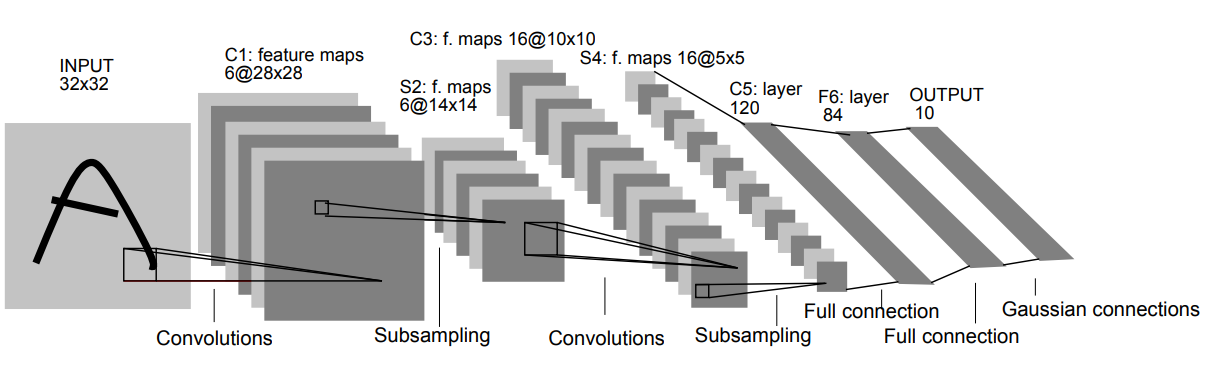
\includegraphics[width=14cm]{img/LeNet-5.png}
    \caption{LeNet-5, CNN for handwritten digits recognition. Source \cite{GradientBasedLearningDigitRec}}
    \label{fig:le-net-5}
\end{figure}

\section{Convolution}
\label{sec:convolution}

Convolution operation on a 3D tensor $H \times W \times D$ (2D image with R, G and B channels) applies a kernel, which is usually a $M \times N \times D$ matrix 
($0 \leq M \leq H, 0 \leq N \leq W$), on the top of spatial location $(0, 0, 0)$. Then products of corresponding elements overlapped by the kernel are computed in all $D$ channels and summed to get the result in this location. The next step is to move move the kernel top to bottom and left to right and perform the convolution operation in every spatial location.

Figure \ref{fig:conv-example} illustrates a convolution on an 2D $4 \times 3$ matrix with an $4 \times 2$ kernel and hopefully clarifies the whole concept. The process for the 3rd order tensor is analogical.

\begin{figure}[h]
    \centering
    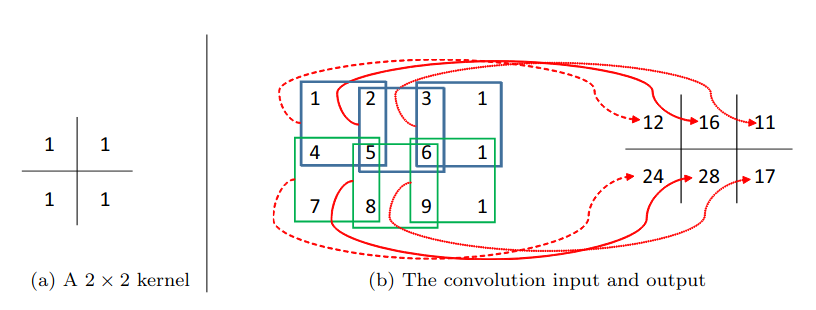
\includegraphics[width=14cm]{img/ConvExample.png}
    \caption{Convolution operation. Source \cite{Wu2017IntroductionTC}}
    \label{fig:conv-example}
\end{figure}

\subsection{The purpose of convolution}
\label{sub:purpose-of-convolution}

Applying convolutions with different kernels, also called \emph{feature extractors}, enables do detect certain set of features from the image. The \ref{fig:conv-lenna} shows effect of applying a $3 \times 3 \times 3$ kernel

\begin{equation}
    K = \begin{bmatrix}
            1 & 2 & 1 \\
            0 & 0 & 0 \\
            -1 & -2 & -1
        \end{bmatrix}
\end{equation}

and a transposed $K^T$ on probably the most processed woman on the internet, Lenna. This particular kernel detects and apmplifies horizontal or vertical edges, but any type of kernel can be used. The next layer is usually a ReLU, which activates only for edges at a certain direction. Subsequent layers in network can activate for more complex group of features or even the entire objects like human face, cat or dog. 

Another advantage of convolution layer is that it is \emph{spatially invariant}, which means that it is insensitive to feature position on a picture. If there were many objects at the same image, the feature would activate at multiple locations. What is more, the convolution network architecture encourages a parameter sharing. If the network learned to recognize an eye or a hand, it does not need to limit it to one particular type of eye (e.g. human eye). Instead the bottom layers may share patterns used to detect more abstract features in the next layers. In our example, the eye pattern can be used to detect a human, a cat or a dog.

All in all, convolution kernels combined with a deep and hierarchical structures are en extremely efficient tool for visual recognition tasks.

\begin{figure}[h]
    \centering
    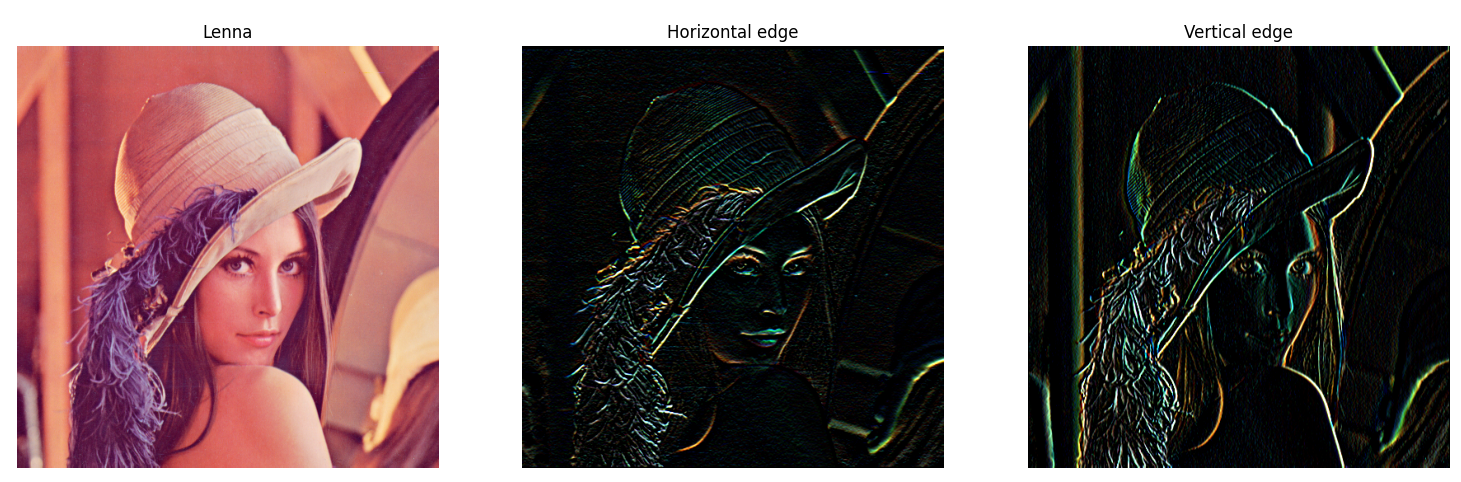
\includegraphics[width=16cm]{img/Lenna1.png}
    \caption{The Lenna image and the output of different convolution kernels}
    \label{fig:conv-lenna}
\end{figure}

\section{Activation}
\label{sec:conv-activation}

CNN adopted three main activation functions: \textbf{sigmoid}, \textbf{ReLU} and \textbf{PReLU}, shown at \ref{fig:conv-activation}. They have been described in \ref{sec:activation-function}, except the PReLU which is a parametric version of ReLU and is described in the appendix to this section.

\begin{figure}[h]
    \centering
    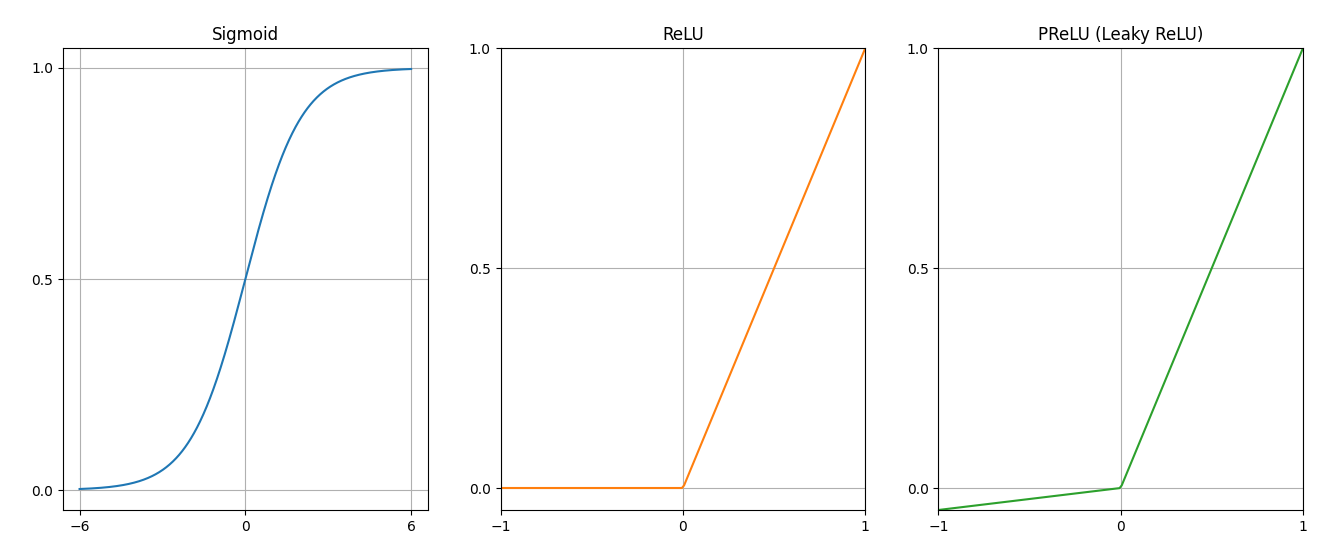
\includegraphics[width=16cm, height=6cm]{img/CNN-activations.png}
    \caption{Non-linear activations adopted by CNNs}
    \label{fig:conv-activation}
\end{figure}

Every of them serve clip the output of convolution. Sigmoid squashes the output into the $[0, 1]$ interval. The ReLU sets the negative values to 0 and keeps the positive unchanged. The PReLU maps larger negative values to smaller ones by reducing the slope or the mapping function. It has been shown in the experiments that removing a non-linear operation significantly decreases the performance of CNN. Their importance have been described by \emph{C.-C. Jay Kuo} \cite{kuo2016understanding}, \emph{Kaiming He et al.} \cite{he2015delving} and many others.


\subsubsection*{PReLU}
\label{sub2:prelu}

The \textbf{Parametric Rectifier Linear Unit} function has been introduced in \emph{Delving Deep into Rectifiers: Surpassing Human-Level Performance on ImageNet Classification} \cite{he2015delving}. The authors of the publication state that using this particular activation they managed to outperform human at image recognition of \emph{ImageNet} \footnote{1000-class ImageNet 2012 dataset} dataset.

The function is defined as

\begin{equation}
    f(y_i) = 
        \begin{cases}
        y_i & y_i > 0 \\
        a_i y_i & y_i \leq 0
        \end{cases}
\end{equation}

where $y_i$ is the activation input on the \emph{i-th} channel and $a_i$ is the coefficient controlling the slope of the negative part. 

\section{Pooling}
\label{sec:conv-pooling}

This layer is mainly responsible for a shift invariance and spatial dimension reduction. In other words, a processed image has a reduced size containing only detected features by the previous layers. This reduces the calculations complexity and enables the network to focus only on important parts of an image, dropping the remaining part. If the task was to find a Wally, there is no need to keep track of information about the location where he stands.

Originally, pooling was performed by \textbf{subsampling} layers. Neurons receive an input from a small non-overlapping receptive field of a previous layer. Then each neuron computes a sum of its inputs, multiplies it by a trainable coefficient, adds a trainable bias and passes the result through non-linear transfer function. Such approach was implemented in \emph{LeNet-5} \cite{GradientBasedLearningDigitRec}.

\begin{equation}
    a_j = tanh\left(\beta \sum_{N \times N} a_i^{N \times N} + b \right)
\end{equation}

Recently, subsampling layer has been replaced by \textbf{max pooling} operation. It is much simpler in foundations since it only propagates the maximum of the receptive field to the next layer. Despite that, as \emph{Dominik Scherer et al.} \cite{MaxPool} showed, it is superior for capturing invariances in image data to a subsampling operations.

\begin{equation}
    a_j = \max_{N \times N} \left( a_i^{N \times N} u(n, n) \right)
\end{equation}

Where $u(x, y)$ is a transfer window function. In both cases the output is a lower resolution image.

\section{Flattening}
\label{sec:flattening}

\section{Full Connection}
\label{sec:full-conn}
	\chapter{Reinforcement Learning}
\label{cha:reinforcement-learning}

Having discussed ANN and CNN it is high time to introduce third and last component used in the vision system for autonomous boat control. Reinforcement learning is a machine learning training method based on reward-penalty system. The agent is put in the environment with a defined \textbf{action space} and \textbf{state space} \ref{sub:mdp}. The agent is rewarded for taking an action which leads closer to desired state and punished with a negative reward for an undesired behaviour. Value of every action is remembered. This programs the agent to seek a long-term and maximum overall reward in order to achieve an optimal solution.

\section{Reinforcement Learning Methods Taxonomy}
\label{sec:classification-of-reinforcement-learning-methods}

Before diving into details of Q-learning algorithm used in the vision system project, let us give a brief overview over different types of RN methods. The notation introduced in this section is used in further parts of the paper.

\subsection{Policy}
\label{sub:policy}

The policy is a strategy used by the agent to achieve desired goal. It dictates which action is going to be taken based on agent's state and the environment. Formally the policy $\pi(s)$, $s\in{S}$, is defined in terms of the \emph{Markov Decision Process} \ref{sub:mdp} to which it refers. 

\subsubsection*{Off-Policy}
\label{sub2:off-poicy}

% TODO: Q-value reference
% TODO: Q-learning referece
In an off-policy algorithm the agent state and the action that will be taken is evaluated regardless of the currently followed policy $\pi$. Q-learning is an example. It updates its Q-values using Q-value of the next state $s'$ and the greedy action $a'$. That is, the return for state-action pairs is estimated assuming that a greedy policy was followed even though the agent is not following the greedy policy.

\subsubsection*{On-Policy}
\label{sub2:on-policy}

On the other hand, an on-policy algorithm evaluates which action agent should take with respect to the policy it follows. For example, SARSA is an algorithm which updates its Q-values using Q-value of the next state $s'$ and the current policy's action $a''$. The return for state-action pairs is estimated assuming that the current policy is followed in the next state.

\subsection{Model}
\label{sub:model}

Model is in simple terms the behaviour of an environment. Based on whether the agent needs to know such model to determine a policy RN algorithms can be classified to two groups. There are two main types of networks regarding the model.

\subsubsection*{Model-Free}
\label{sub2:model-free}

A model-free algorithm does not have to learn the model to evaluate its policy. One of the most common examples is \emph{Q-learning}, but such approach is also used in \emph{Actor-critic} or \emph{Policy gradient} methods which search directly over policy space to find policies that result in a better reward from the environment.

\subsubsection*{Model-Based}
\label{sub2:model-based}

A model based algorithm must know the model of an environment before finding an optimal policy. Therefore a value of the next step can be predicted without actually performing that step. \mbox{AlphaGO} (\ref{sub:intro-games}) is an perfect example.

\subsection{Base}
\label{sub:base}

This \textbf{Value-based} network does not store explicitly the policy. Instead, it keeps track only of a value function. The policy can be derived directly from the value function, which means taking an action which corresponds to the best value.
The opposite approach is taken in \textbf{Policy-based} methods, where the representation of the policy $\pi(s)$ is created explicitly and kept in memory during the learning process. 

\section{Q-learning}
\label{sec:q-learn}

In a classical reinforcement learning action $a$ the agent should take is determined by the value $V(s')$ of the next state. Q-learning approach focuses on the quality of the action $Q(s, a)$ instead. It is an off-policy, model-free algorithm used in many reinforcement learning solutions.

\subsection{Bellman Equation}
\label{sub:bellman-eq}

This is the underlying principle of the Q-learning algorithm, first introduced by \emph{Richard Bellman} \cite{Bellman:DynamicProgramming}.

\begin{equation}
    V(s) = \max_a\left(R_a(s, s') + \gamma V(s') \right)
\label{eq:bellman}
\end{equation}

Where $V(s)$ is the value of a given state, $R(s, a)$ is a reward for taking an action $a$ in a state $s$ and $\gamma$ is a discount factor. The equation is straightforward, all it tells that a value of a given state is assessed based on an action for which the sum of a reward and discounted value of the next state is maximal. The assumption is that the value of the next state must be known. To put it in simpler terms, an agent which wants to know how good (or bad) its current state is, looks around for opportunities. If there is a happy place around, then the value of current state is high. If you were one step from reaching the top of the Mount Everest, you would perhaps be more excited than if you were looking at it on a postcard.

\subsection{Markov Decision Process}
\label{sub:mdp}

Markov Decision Process can be expressed as a tuple $(S, A, P_a, R_a)$, as stated in \emph{Markov Decision Processes: Concepts and Algorithms} \cite{Otterlo2012MarkovDP}:

\begin{itemize}
    \item $S$ is a state space, a set of all possible states of the agents,
    \item $A$ is an action space, a set of all the behaviors agent can take,
    \item $P_a(s, s') = P(s_{t+1} = s' | s_t = s, a_t = a)$ is the probability that the outcome of an action $a$ taken in state $s$ will be state $s'$ at time $t+1$,
    \item $R_a(s, s')$ is the reward received after transition from state $s$ to state $s'$ after taking action $a$.
\end{itemize}

The key concept behind MDP is that the outcome of an action is independent to previous actions and states. It only depends on a current state. The current state $s$ must give sufficient information to make an optimal decision. A policy $\pi^{*}(s)$ which for every state $s$ results in an optimal decision is called \emph{optimal policy} and can be defined as 

\begin{equation}
    V^{\pi^{*}}(s) \ge V^{\pi}(s)
\end{equation}

for every $s \in S$ and all policies $\pi$.

In realty, when agent takes a particular action it does not ensure that it will end in a desired state. Although it has control over all actions, there environment can still affect them in a unexpected way. Taking a boat as an example, propellers speed may be set to make it turn right, but a sudden wave might move the boat left anyway. That is why the transition in MDP is expressed in terms of probability. Having that in mind, we can write the Bellman equation (\ref{eq:bellman}) in terms of \emph{expected value}:

\begin{equation}
    V^{*}(s) = \max_a \sum_{s'} P_a(s, s') \left(R_a(s, s') + \gamma V^{*}(s') \right)
\label{eq:state-value}
\end{equation}

To select an optimal action given the optimal value function $V^{*}$:

\begin{equation}
    \pi^{*}(s) = arg \max_a \sum_{s'} P_a(s, s') \left(R_a(s, s') + \gamma V^{*}(s') \right)
\label{eq:state-value-policy}
\end{equation}

This is a \emph{greedy policy}, since the best action is always chosen based on the value function $V$.

\subsection{Q-value}
\label{sub:q-val}

Q-value can be described as \emph{quality of the action} $a$. The state-action value function $Q$ becomes an decision making indicator instead of state value function $V$. This slight change has considerable consequences. Since there is no longer need to compute the value of the next state, an algorithm becomes independent to the model. That is, the agent can take a step without prior knowledge of the properties of the incoming state. The action-state equation analogous to \ref{eq:state-value}:

\begin{equation}
    Q^{*}(s, a) = \sum_{s'} P_a(s, s') \left(R_a(s, s') + \gamma \max_{a'} Q^{*}(s', a') \right)
\label{eq:q-value}
\end{equation}

The relation between $Q$ and $V$ is given as following:

\begin{equation}
    V^{*} = \max_a \left(Q^{*} (s, a)\right)
\end{equation}

and analogously to \ref{eq:state-value-policy}

\begin{equation}
    \pi^{*}(s) = arg \max_a Q^{*}(s, a)
\end{equation}

The above equation states that the best action is the one that has the highest return from possible states resulting from taking that action.
In other words, the agent chooses an action which leads to a state which gives the most opportunities to progress. It is like deciding between universities to apply for, assuming you are eligible for admission to every, you would perhaps choose the most prestigious one.

\subsection{Exploration-exploitation}
\label{sub:exploration-exploitation}

The ultimate goal of a Q-learn algorithm is to obtain the optimal policy $\pi^{*}$, but the difficulty is that the model of the environment is unknown. In order to collect missing pieces of information, the agent has to \emph{explore} what is the universe that it has been put into. As interesting as it may be, exploration itself will not bring the agent closer towards finding a desired state $s$ and thus learning the optimal policy. The only way to increase a total reward is to \emph{exploit} the current knowledge about best possible actions. However, there may a better, yet unknown action which only can be discovered in the exploration process. Finding the balance between \emph{exploration} and \emph{exploitation} is crucial for every RN algorithm.

The most rudimentary strategy is \emph{$\epsilon$-greedy} policy. Given the $\epsilon \in [0, 1]$, the agent takes its current best action $arg\max_a Q(s, a)$ with a probability $(1 - \epsilon)$ and a randomly selected action $a \in A$ with probability $\epsilon$. There are obviously more sophisticated strategies to balance between exploration and exploitation, but the Deep-Q-learning \ref{sec:deep-q-learn} algorithm used in the final project is based on this one. Therefore there is no need to introduce additional methods.

\subsection{Temporal Difference Learning}
\label{sub:temporal-difference-learning}

This is a heart of Q-learning algorithm. One could think of two approaches of finding the intermediate values $Q(s, a)$ which eventually lead to desired state $s$. First possibility is to wait until the end of an episode and reward or punish actions taken along the path. For a complex model it would require considerable amount of memory. Luckily there exists a more efficient way. Instead of sitting patiently until the very end and then act, the q-value can be updated at every step using a \emph{temporal difference}.

It was well described by \emph {Richard S. Sutton} \cite{SuttonTD} who wrote a well-depicting analogy. Suppose a weatherman wants to predict on each day of the week a weather on the following Sunday. The conventional way would be to compare the actual outcome to each prediction and then adjust each of them. On the contrary, a temporal difference approach would be to compare each day's prediction with that made on the following day. So if 50\% chance of rain is predicted on Monday, and a 75\% chance on Tuesday, a TD method increases predictions for days similar to Monday. For the Q-learning case is adjusted based on the reward and the estimated discounted value of the next state.

Before diving into mathematics, let us simplify equation \ref{eq:q-value} using an alias,

\begin{equation}
    Q(s, a) = \sum_{s'} P_a(s, s') \left(R_a(s, s') + \gamma \max_{a'} Q(s', a') \right)
    \equiv
    R_a(s, s') + \gamma \max_{a'} Q(s', a')
\label{eq:q-learn-alias}
\end{equation}

and introduce a virtual timer $t$ representing each iteration the agent acts.

Before performing an action, there is some $Q(s, a)$ value known for a transition between current state $s$ and the next $s'$. The agent then performs the action and it turns out that the outcome q-value equals \[R_a(s, s') + \gamma \max_{a'} Q(s', a')\]
An cautious reader may notice that it is simply an above equation \ref{eq:q-learn-alias}. The detail that matters is time. First one is just an expectation and the latter a reality. Temporal difference is simply a neat way to express it,

\begin{equation}
    TD = R_a(s, s') + \gamma \max_{a'} Q_{t}(s', a') - Q_{t-1}(s, a)
\label{eq:temporal-difference}
\end{equation}

It is directly used to update the $Q_t(s, a)$ after taking an action,

\begin{equation}
    Q_t(s, a) = Q_{t-1} + \alpha TD_t(s, a)
\end{equation}

The $\alpha$ factor, called a \emph{learning rate}, is used because do not live in a perfect world, unless you are reading it in a distant future where all diseases are gone. The action taken might have been with some likelihood unexpected or random because of stochastic environment. Therefore, instead of replacing the old $Q_{t-1}$ with the new $Q_t(s, a)$ we update it with a pace controlled by $\alpha$.

\vspace{.5cm}

Finally, the Q-learning algorithm can be written as following,

\begin{lstlisting}[language=Python, caption={Q-learning algorithm}]
    gamma = x
    alpha = y
    init_q_values()
    for e in episodes:
        s = starting_state
        while s != final_state:
            action = choose_action()
            new_state, reward = take_action(action)
            Q(s, a) = Q(s, a) + alpha*TD
            s = new_state
\end{lstlisting}

Such value iteration algorithm converge to the optimal action-value function $Q^*$.

\section{Deep Q-learning}
\label{sec:deep-q-learn}

Q-learning appears to be a great algorithm for simple reinforcement learning tasks. However, it struggles for more complex environments. One of the reasons is that it explores too slowly and learns only from the consequent states, which may by highly correlated. Fortunately, deep neural networks come with support. Their ability to learn complex patterns comes in handy for a decision-making process in a more sophisticated environment. Instead of TD, the neural network is used to update $Q(s, a)$. The architecture of DNN is straightforward. Input layer consists of \textbf{observations} which are all the information that an agent retrieves from the environment. Then there are $N$ hidden layers and finally the output layer made of possible q-values $Q_1(s, a_1), Q_2(s, a_2), ..., Q_x(s, a_x)$, where $x$ is a number of available actions.

\vspace{1cm}

\begin{figure}[h]
\centering
\begin{tikzpicture}
\foreach \i in {1, ..., \inputnum}
{
    \node[circle, minimum size = 6mm, draw=black] (Input-\i) at (0, -\i) {};
}

\foreach \i in {1, 2, ..., \hiddennum}
{
    \node[circle, minimum size = 6mm, draw=black, yshift=(\hiddennum-\inputnum)*5mm] (Hidden-\i) at (2.5, -\i) {};
}

\foreach \i in {1, ..., \outputnum}
{
    \node[circle, minimum size = 6mm, draw=black, yshift=(\outputnum-\inputnum)*5mm] (Output-\i) at (5, -\i) {};
}

\foreach \i in {1, ..., \inputnum}
{
    \foreach \j in {1, ..., \hiddennum}
    {
        \draw[->, shorten >=1pt] (Input-\i) -- (Hidden-\j);
    }
}

\foreach \i in {1, ..., \hiddennum}
{
    \foreach \j in {1, ..., \outputnum}
    {
        \draw[->, shorten >=1pt] (Hidden-\i) -- (Output-\j);
    }
}

\foreach \i in {1, ..., \inputnum}
{
    \draw[<-, shorten <=1pt] (Input-\i) -- ++ (-1, 0)
        node[left]{$observation_{\i}$};
}

\foreach \i in {1, ..., \outputnum}
{
    \draw[->, shorten <=1pt] (Output-\i) -- ++(1, 0)
        node[right]{$q_{\i}$ vs $q_{target\i}$};
}
\end{tikzpicture}
\caption{En example of simple Deep-Q-Network}
\label{fig:deep-q-network}
\end{figure}

The network learns through comparison of each $q_1, q_2, ..., q_n$ with \emph{target} q-values. These are the values remembered from previous steps for taking an action $a$ from the same state $s_{past} = s_{current}$. Then loss\footnote{Loss and cost function are used interchangeably in most cases. Precisely a loss function is for a single training example whereas cost function is the average loss over the entire training dataset} (\ref{sec:cost-function}) is calculated and backpropagated through the network to update all the weights and biases. An example of used loss function is \emph{Mean Squared Error} described in \ref{sub2:cost-function-examples}. Then action is selected based on chosen \emph{action selection policy}. The most commonly used are \emph{$\epsilon$-greedy} (\ref{sub:exploration-exploitation}) or \emph{softmax}, but there have been also different policies proposed \cite{AdaptiveEGreedy}.

\subsection{Experience Replay}
\label{sub:experience-replay}

Deep-Q-learning agents constantly update the value function while observing a stream of experience. As most of us, they learn from their mistakes. In their simplest form, agents drop incoming data immediately after a singe update. This is a naive approach though. If one got stuck in an elevator ten times in a row, they would memorize that it is not the brightest idea to enter it the next time, even though it happened to them ten out of thousands elevator rides. Another example of undesired consequence of instant experience replacement would be a chef who is always covered in tears while cutting an onion except that one time that he cut the bottom last\footnote{This is a real life tip}. The possibly useful rare experiences are instantly forgotten and cannot be used in the future.

\emph{Tom Schaul et al.} \cite{schaul2015prioritized} mentions two main issues of learning without an \emph{Experience Replay}:

\begin{itemize}
    \item Strongly correlated parameters update that break i.i.d. assumption of many popular stochastic gradient-based algorithms.
    \item Rapid forgetting of possibly rare experiences that would be useful later on.
\end{itemize}

Experience replay is a remedy for both. An experience memory is simply a buffer which stores last $M$ transitions. $M$ is a size of a memory buffer and transition is expressed as a tuple

\begin{equation}
    \left(s, a, R_a(s, s'), s'\right)
\end{equation}

Every time parameters are updated instead of comparing to the last experience, transitions are \textbf{uniformly} sampled from a memory buffer. Such sample is usually called a \emph{batch} which size depends on the DQN implementation. By learning from the batch of past experiences temporal correlations get broken and rare experiences may be used more than once. Replay memory could be depicted as a sliding window which follows an agent and contains all its valuable memories. 

	\printbibliography

\end{document}
